\documentclass{article}

% Language setting
% Replace `english' with e.g. `spanish' to change the document language
\usepackage[spanish]{babel}

% Set page size and margins
% Replace `letterpaper' with `a4paper' for UK/EU standard size
\usepackage[letterpaper,top=2cm,bottom=2cm,left=3cm,right=3cm,marginparwidth=1.75cm]{geometry}

% Useful packages
\usepackage{amsmath}
\usepackage{graphicx}
\usepackage{enumitem}
\usepackage{comment}
\usepackage{wrapfig}
\usepackage[colorlinks=true, allcolors=blue]{hyperref}

\title{POO Tema 2. Clases y tipos de datos}
\author{Martín González Dios 
\href{https://github.com/martindios}{\includegraphics[height=0.5cm]{github.png}}}

\begin{document}
\maketitle

\section{Tipos de datos primitivos}
Son los \textbf{tipos predefinidos} que tienen correspondencia con los tipos de datos de lenguajes basados en procedimiento (como C). Tiene tamaño fijo, correspondencia directa con los tipos representables en un computador, no tienen métodos y se les reserva memoria en la declaración. \\ 
No son clases, sino que están vinculados a los valores de las variables. Para ser consistentes en el paradigma de la programación orientada a objetos se definen \textbf{wrappers} que envuelven los valores de los tipos en distintos tipos de objetos y proporcionan métodos (obtener el dato, convertiro a texto o convertir a otro tipo primitivo).

\section{Wrappers}
El uso de wappers hace el \textbf{código más complejo}, pero \textbf{el autoboxing y el unboxing permiten tratar un wrapper como si fuese un tipo de dato primitivo o una clase}, utilizamos tipos primitivos como si fueran clases sin problema. 
\begin{itemize}
    \item Autoboxing: convierte un tipo de dato primitivo a un objeto del wrapper correspondiente.
    \item Unboxing: convierte un objeto de un wrapper al tipo de dato correspondiente.
\end{itemize}

Por lo general se prefieren usar tipos primitivos para hacer el código más sencillo. \textbf{Se aconseja utilizar wrappers en las conversiones entre tipos de datos}, especialmente en el manejo de cadenas de texto.

\newpage

\section{Referencias}
\textbf{Los nombres de los objetos son referencias a su posición de memoria}.

\begin{figure}[h]
    \centering
    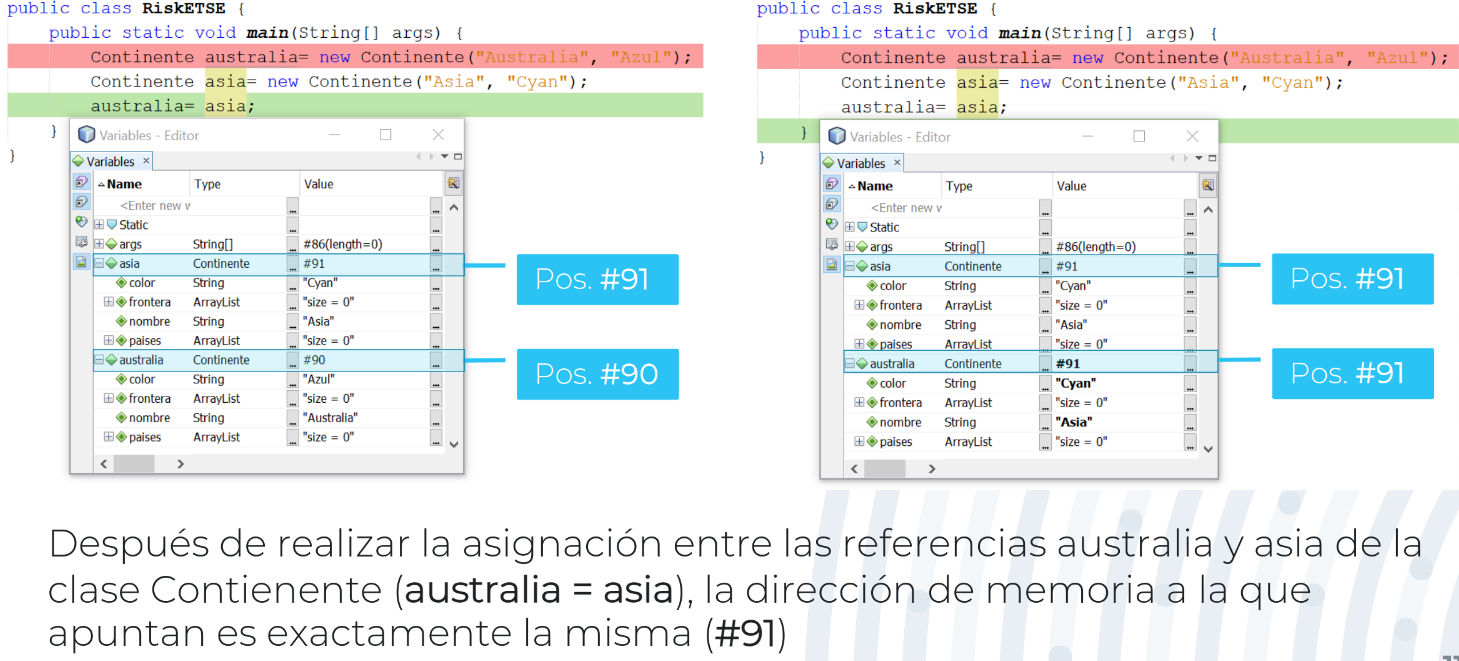
\includegraphics[width=\textwidth]{img-t2/img_279_25.png}
\end{figure}

La \textbf{asignación de memoria entre objetos de denomina aliasing}, esta asignación \textbf{evita la encapsulación de los datos}, permitiendo modificar atributos desde métodos de otras clases. Además, los programas con aliasing son más difíciles de mantener, pues los atributos del tipo objeto se podrían modificar desde cualquier parte del programa. Pero el hecho de \textbf{evitarlo totalmente reduciría mucho el rendimiento}, teniendo que hacer copias completas de unas zonas de memoria a otras.  \\

La dificultad de no usarlo lleva a \textbf{seleccionar zonas de código donde se debe evitar}. La única forma de evitarlo es generando manualmente una nueva referencia del objeto (crearlo) para lo que Java tiene el \textbf{método clone}. Este genera una \textbf{copia exacta del objeto en una posición diferente}, pero debe ser \textbf{implementado explícitamente para cada clase}.

\section{Máquina virtual de Java}
\textbf{Java es un lenguaje interpretado cuya ejecución corre a cargo de la máquina virtual de Java}.

\begin{figure}[h]
    \centering
    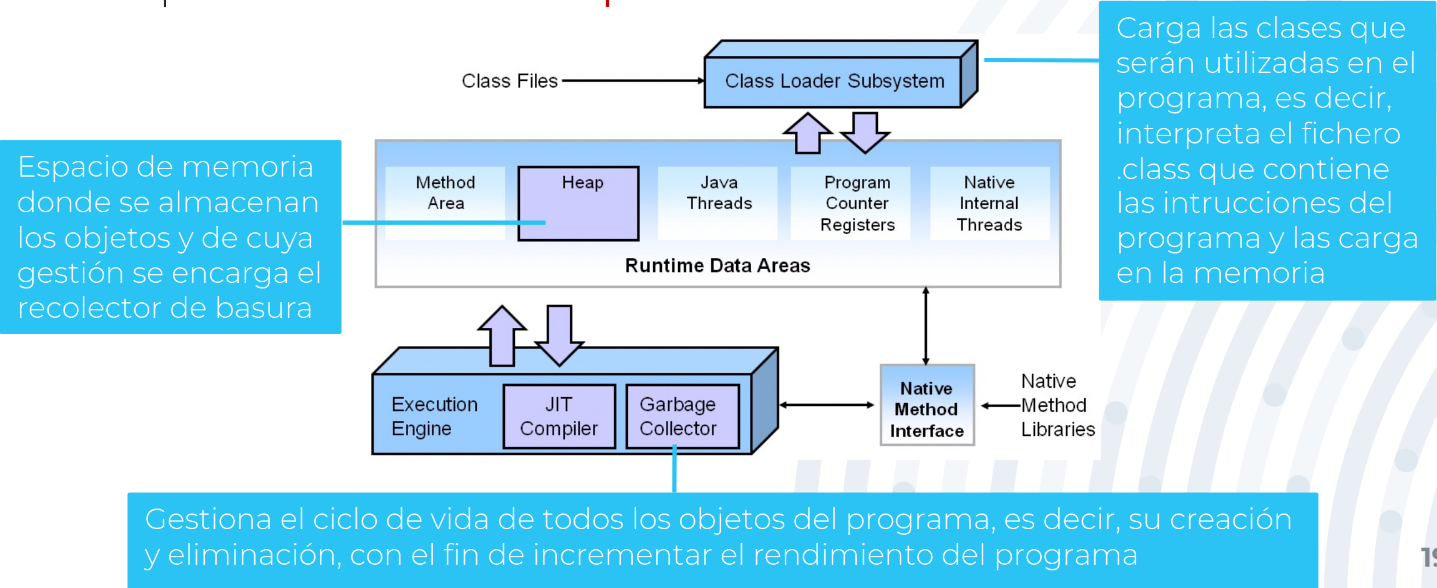
\includegraphics[width=\textwidth]{img-t2/img_318_59.png}
\end{figure}

\newpage

\section{Almacenamiento}

\subsection{Datos}
\begin{itemize}
    \item \textbf{Pila (stack)}: zona de la memoria a la que el procesador tiene acceso directo con el puntero pila. La lectura y escritura es rápida y eficiente. \textbf{Las variables existen en ella solo en la ejecución del método que las creó, luego se eliminan}. \\
    El compilador debe saber la memoria que se va a necesitar para mover el puntero, por lo que los datos en ella deben tener un tamaño conocido, es decir, se necesita saber el código de los métodos, datos primitivos usados durante la ejecución y referencias a objetos creados.

    \item \textbf{Montón (heap)}: zona de la memoria de la que no se conoce el tamaño ni el tiempo que van a estar disponibles los datos (dinámica). \textbf{Almacena objetos creados en la ejecución}. El rendimiento de un programa Java está muy ligado con la gestión eficiente del montón, que la lleva el recolector de basura, pues los datos no se eliminan automáticamente cuando dejan de ser necesarios.
\end{itemize}

\subsection{Métodos}
Una clase no ocupa memoria, \textbf{las instrucciones de los métodos se cargan en la pila al crear un objeto de esa clase}, a partir de eso se puede acceder a todos los métodos a través del objeto y del operador “.”. \\
Del mismo modo podemos acceder al valor de los atributos de ese objeto.

\section{Recolector de basura}
\textbf{Busca en la memoria del programa objetos que no se encuentran en uso para eliminarlos}. Es un proceso que se lanza durante la ejecución en segundo plano, mejorando el rendimiento al facilitar el acceso a objetos que se están usando y no a los eliminados, además de ser más eficiente con la memoria. \\

\begin{enumerate}
    \item \textbf{Marcado}: identifica las zonas de la memoria que están siendo muy usadas (muy ineficiente si se analizan todos los objetos del sistema).

    \item \textbf{Borrado normal}: eliminan los objetos que llevan más tiempo sin referencia asignada.

    \item \textbf{Borrado con compactación}: además de eliminar los objetos los mueve los que quedan en memoria a posiciones consecutivas. 
\end{enumerate}
Las operaciones de marcado y compactación son muy ineficaces ya que se ejecutan continuamente.

\newpage

Generalmente el uso y eliminación de objetos no es uniforme en el tiempo, a medida que pasa el tiempo se mantienen menos objetos en la memoria. Para facilitar la gestión de vida de los objetos se puede dividir la memoria en generaciones. 

\begin{figure}[h]
    \centering
    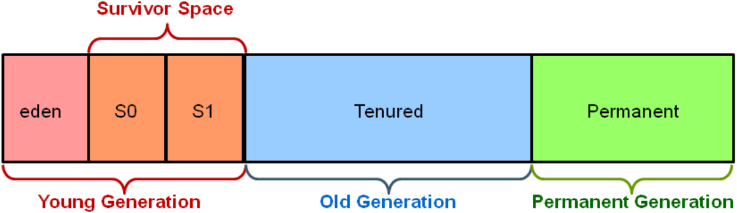
\includegraphics[width=0.65\textwidth]{img-t2/img_314_39.png}
\end{figure}

\begin{itemize}
    \item \textbf{Young generation}: se almacenan y se le asigna una fecha a todos los objetos. Cuando se llena, se lanza una recolección de basuar menor (donde los threads se paran), muy rápida, los objetos que no se eliminan envejeces y pasan a old generation.

    \item \textbf{Old generation}: se almacenan los objetos de larga duración, los que tienen una edad mayor que la umbral. Cuando se llena, se lanza una recolección de basura mayor (donde los threads se paran), que es mucho más lenta, pues involucra todos los objetos vivos.

    \item \textbf{Permanent generation}: almacena las clases y los métodos, se llena en la ejecución con metadatos de las clases (carga dinámica). A partir de Java 8 se sutituyó por metaspace.
\end{itemize}

Inicialmente la young generation está vacía, cualquier objeto recién creado se almacena en el eden. Cuando se llena se lanza una RB menor, eliminando los elementos con referencia null, el resto pasan a S0. En el siguiente RB menor, los objetos usados del eden se mueven al espacio S1, los objetos usados del objeto S0 se mueven al espacio S1 aumentando su edad, y se eliminan del espacio S0 los objetos no usados. En cada RB menor se comprueba si los objetos superan la edad umbral y si es el caso promocionan.

\section{Referencias}

\subsection{Gestión avanzada}
Existen 4 tipos de referencias:
\begin{enumerate}
    \item \textbf{Referencias fuertes}: por defecto, se crean al instanciar un objeto, hasta que apuntan a null el recolector de basura no los elimina. A esta referencia se accede con .get().

    \item \textbf{Referencias débiles}: debe instanciarse la clase WeakReference, se eliminan cuando no apuntan a una referencia fuerte o apuntan a null.

    \item \textbf{Referencias suaves}: debe instanciarse la clase SoftReference, se eliminan solo cuando es necesario tener memoria.

    \item \textbf{Referencias fantasma}: debe instanciarse la clase PhantomReference, están pensadas para acceder a memoria cuando las referencias fuertes no están disponibles, pues la referencia se guarda en un cola a la que se accede con queue.poll().
\end{enumerate}

Las \textbf{referencias suaves y fantasma} se utilizan para hacer cachés en memoria y poder acceder a referencias fuertes que ya no están disponibles en memoria. Las \textbf{débiles} para acceder dinámicamente a la referencia fuerte hasta que ya no esté disponible y así evitar el aliasing.

\newpage

\subsection{Clase String}
Podemos \textbf{crear Strings directamente} (String str = “abc”), se guardan en el String Pool del montón y si se asigna la misma cadena de texto a otra referencia apuntan a la misma dirección, \textbf{o indirectamente} (String str = new String(“abc”)), se guarda en el montón fuera del String Pool aunque exista la cadena. \\

\textbf{Una cadena de texto es un objeto inmutable} (no se puede modificar tras reservar memoria y asignarle valor). Su uso indiscriminado puede bajar mucho el rendimiento. \textbf{Si se va a modificar mucho una cadena} no se debería utilizar String, sino un \textbf{String Buffer}, que no reserva memoria cada vez que se genera una cadena de texto.

\section{Identidad de objetos}
\begin{enumerate}
    \item \textbf{Si ambos objetos ocupan la misma posición de memoria podemos decir que son iguales} (condición muy restrictiva, ya que no se están comparando dos objetos, sino que se comparan dos referencias a un mismo objeto).

    \item \textbf{Si ambos objetos son del mismo tipo y los valores de todos los atributos son iguales podemos decir que son iguales} (deben tener los mismos valores de los atributos en ese momento y ser inmutables).
\end{enumerate}

El \textbf{método equals indica si dos objetos son iguales}. La implementación heredada de Object solo compara referencias, por lo que se debe \textbf{reimplementar el método en cada clase}. \\
Todos los métodos con los que se realizan comparaciones deben tener el método equals implementado. \textbf{Los atributos utilizados en equals para definir la igualdad entre objetos deberían ser primitivos, wrappers a primitivos o cadenas de texto}.

\begin{comment}
\begin{figure}[h]
    \centering
    \includegraphics[width=0.5\textwidth]{1.png}
    \caption{}
\end{figure}
\end{comment}

\begin{comment}
\begin{wrapfigure}[]{r}{0.5\linewidth}
    \centering
    \includegraphics[width=\linewidth]{8.png}
    \caption{}
\end{wrapfigure}
\end{comment}

\end{document}